\section{Introduction}

\begin{figure}[h]
   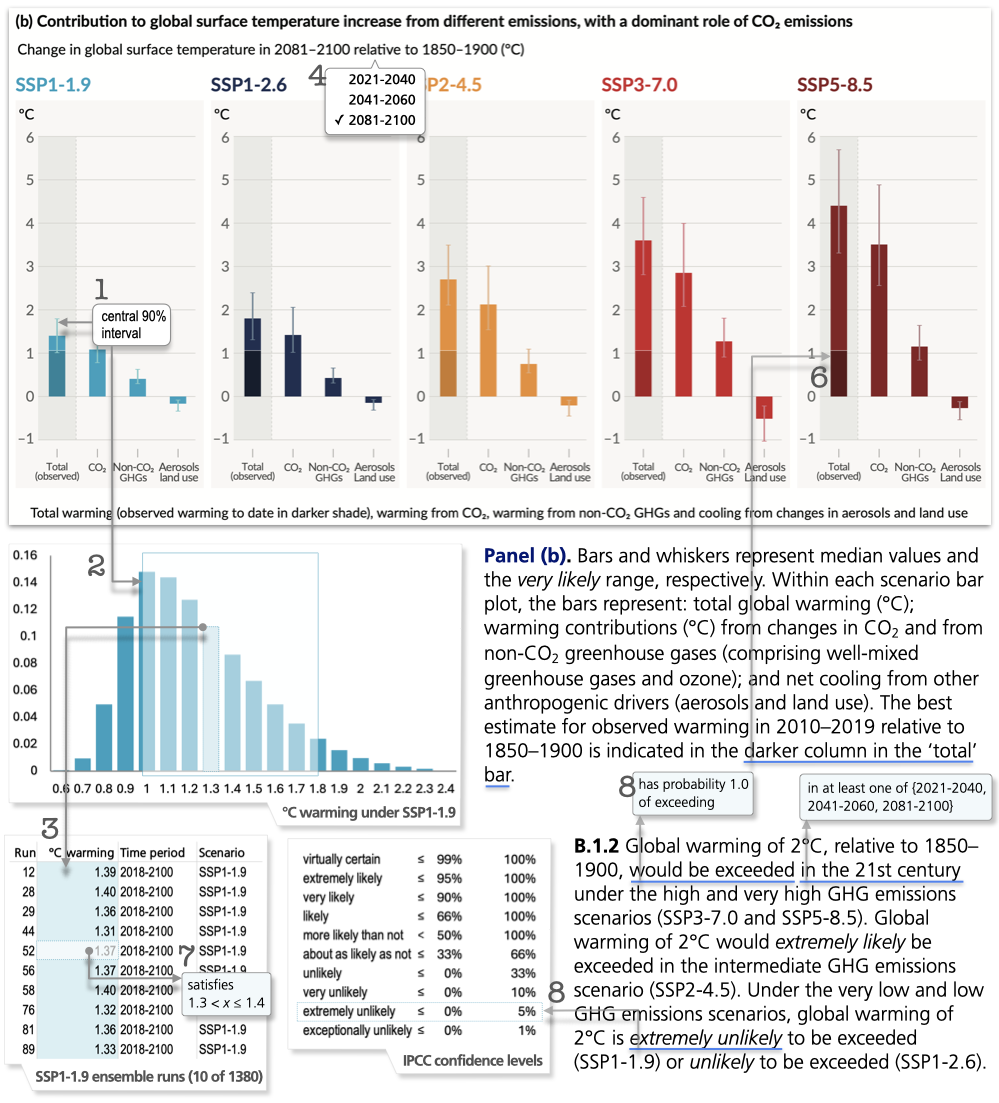
\includegraphics[width=0.9\textwidth]{fig/ipcc-mockup.png}
   \caption{Mockup of end-user transparency features (numbered 1 to 8)}
   \label{fig:ipcc-mockup}
\end{figure}

\subsection{Self-Certifying Text}
Examples of text we might want to link or interpret semi-formally/quantitatively:

\begin{itemize}
\item Quantitative expressions
\begin{itemize}
   \item pure numerical values
   \item percentages
   \item rounded or normalised numbers
\end{itemize}
\item Graded Adjectives (e.g.~\emph{virtually certain}, \emph{exceptionally unlikely})
\item References to visual elements and their parts (mereology)
\end{itemize}
